\documentclass[12pt]{article}
\usepackage{indentfirst}
\usepackage{braket}
\usepackage{color}
\usepackage{graphicx}
\usepackage{graphics}
\usepackage{subfig}
\usepackage{amsmath}
\usepackage{amssymb}
\usepackage{geometry}
\usepackage{float}
\usepackage{ulem}
\usepackage{framed}
\usepackage{empheq}
\usepackage{mathtools}
\usepackage[linkcolor=blue,colorlinks=true,linktoc=all]{hyperref}
\makeatletter
\@addtoreset{equation}{section}
\makeatother
\renewcommand{\theequation}{\arabic{section}.\arabic{equation}}

\graphicspath{{Diagrams/}}
\geometry{a4paper,scale=0.85}
\title{\Large{\textbf{Report for 1D Ising Model\\}}}
\author{\textbf{Roni Bartsch}\\
	Bar-Ilan University\\Guo Liangliang}
\date{}
\begin{document}
	\maketitle
	
	\begin{abstract}
		This report talks the simulation of 1D ising model which there is no external magnetic field ($B=0$) with metropolis algorithm. Behaviours of both ferromagnets ($J=1$) and antiferromagnets ($J=-1$) are studied using the simulated data. What the report mainly considered is how  average magnetization, average energy and specific heat behave with temperature changes. Besides, the dynamics of the system and how it reaches equilibrium are also discussed. The code for the simulation is written with Python and be attached in another file.
	\end{abstract}
	
	\section{Introduction}
	\label{sec: introduction} 
	
	\subsection{Ising Model}
	\label{sec: ising model}
	In statistical mechanics, ising model is used to describe magnetic systems. It consists of a lattice with a discrete value $\sigma _i  \in \{-1,1\}$ assigned to each point, which represents the spin at the lattice site ($\sigma_i=-1$ means spin down, $\sigma_i=1$ means spin up). The Hamiltonian of the system can be given by 
	\begin{align}\label{equ: hamiltonian of ising model}
		H=-\sum_{i,j}J_{i,j}\sigma_i \sigma _j -h \sum_i \sigma_i
	\end{align}
	
	where the first sum is over the interacting spin pairs and the second sum is over the entire lattice. $J_{i,j}$ is the exchange term between the spins and $h$ represents the energy term between the spins and external magnetic field. When $J_{i,j}>0$, the neighbouring spins will tend to arrange to the same direction and the corresponding property is ferromagnetism. If $j_{i,j}$ is negative, the close spins will ten to have oppose directions, the property is antiferromagnetism.  Ferromagnetism occurs in some magnetic materials below the Curie Temperature $T_C$. Spins in microscopic regions (domains) $^{\cite{wikipedia magnetic domain}}$ are aligned. The magnetic field is strong in the domain, but the domains in the material are randomly ordered with respect to one another, the material is usually unmagentised. In the presence of an external magnetic field, the domains will line up with each other which will cause the material to become magnetised.  If the applied field is removed, the domains remain aligned, meaning ferromagnetic materials can exhibit spontaneous magnetisation (remanence): a net magnetic moment in the absence of an external magnetic field. Above the Curie temperature, the thermal motion is sufficient to disrupt the alignment, and the material becomes paramagnetic. 
	
	In this report, we only consider 1D ising model which assumes there is only interactions between nearest neighbour spins, the exchange term is a constant value for all neighbouring pairs of spins $J_{i,j}=J$ (Ferromagnets: $J=1$; Antiferromagnets: $J=-1$) and there is no external magnetic field ($h=0$). So we can get a more simple expression of Hamiltonian compare with equation \ref{equ: hamiltonian of ising model}.
	\begin{align}
		H=-J\sum_{i=0}^{N-1} \sigma_i \sigma_{i+1}
	\end{align}
	
	\subsection{Thermodynamic Variables}
	\label{sec; thermodynamic variables}
	
	For 1D ising model, there is exact solution which can be found at Wikipedia $^{\cite{wikipedia ising model}}$. From that, we can get the analytic function of the thermodynamic variables against temperature, which are 
	\begin{align}\label{equ: analytic solution of variables}
		\nonumber \braket{E(T,B)}&=-J \tanh{\frac{J}{T}}\\
		\nonumber \braket{M(T,B)}&=\frac{\sinh^2{\frac{B}{T}}}{\sqrt{\sinh^2{(B/T)}+e^{-4J/T}}}\\
		\nonumber \braket{\chi(T,B)}&=\frac{e^{-4J/T} \cosh{(B/T)}}{T (\sinh^2{(B/T)}+e^{-4J/T})^\frac{3}{2}}\\
		\nonumber C_V(T,B)&=\frac{J^2 \text{sech}^2{(J/T)}}{T^2}
	\end{align}
	
	And the diagrams are as Figure \ref{fig: analytic solution as temperature}
	\begin{figure}[htb]
		\centering
		\subfloat{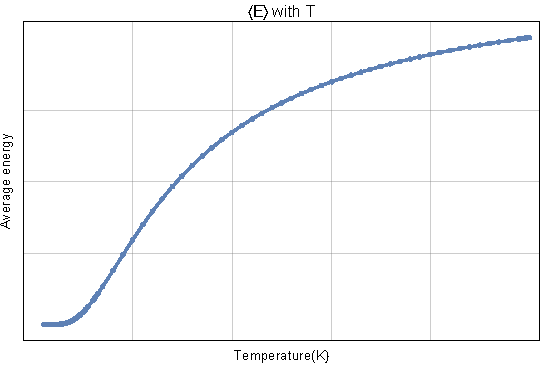
\includegraphics[scale=0.45]{analytic average energy(j=1)}} \quad
		\subfloat{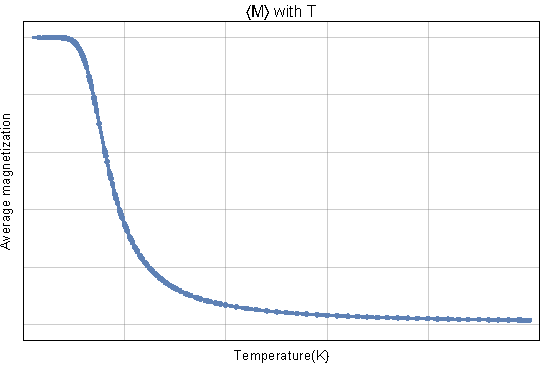
\includegraphics[scale=0.45]{analytic average magnetization(j=1)}} \quad
		\subfloat{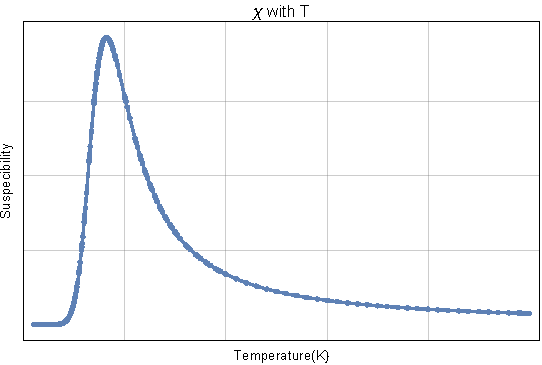
\includegraphics[scale=0.45]{analytic suspecibility(j=1)}} \quad
		\subfloat{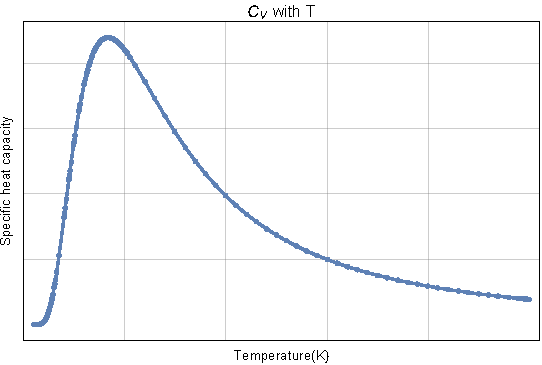
\includegraphics[scale=0.45]{analytic specific heat(j=1)}} \quad
		\subfloat{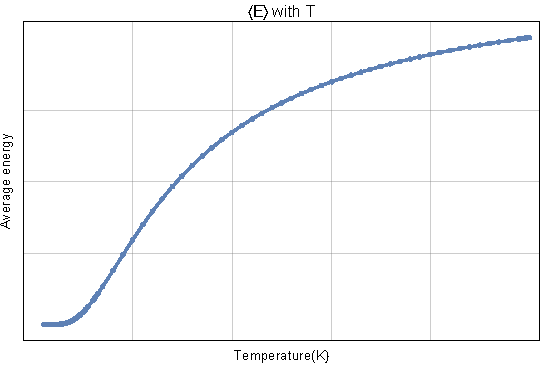
\includegraphics[scale=0.45]{analytic average energy(j=-1)}} \quad
		\subfloat{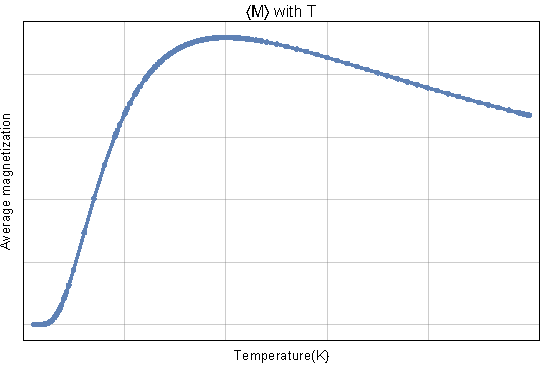
\includegraphics[scale=0.45]{analytic average magnetization(j=-1)}} \quad
		\subfloat{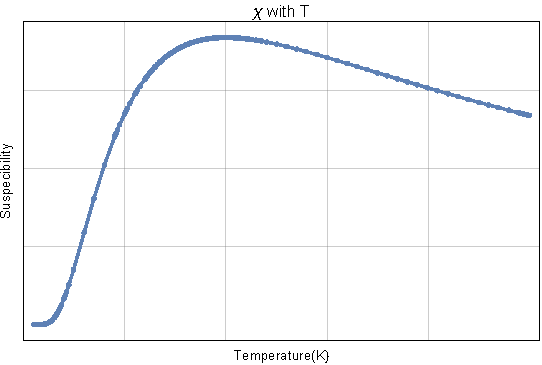
\includegraphics[scale=0.45]{analytic suspecibility(j=-1)}} \quad
		\subfloat{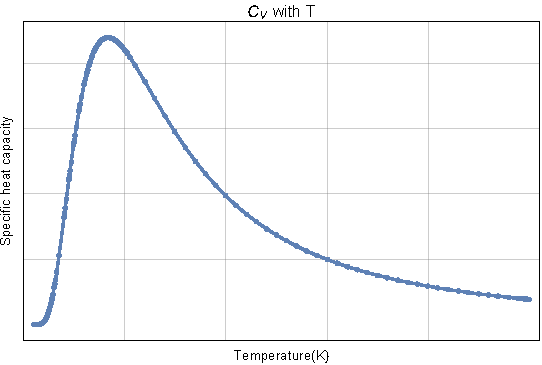
\includegraphics[scale=0.45]{analytic specific heat(j=-1)}} 
		\caption{Exact (per spin) thermodynamic functions for the 1d Ising model. From left to right: $\braket{E},\braket{M},\chi,C_V$ with the temperature changes. Top Row means ferromagnets($J=1$), under row means antiferromagnets($J=-1$). \textcolor{blue}{To be noted, the plots is based on external field $B=0.01$, that is because when $T\neq0$, $\braket{M(T,B)}$ is always zero for $B=0$,  which can't tell us any information.So these diagrams are just samples, the simulated data can have difference.}}
		\label{fig: analytic solution as temperature}
	\end{figure}
	
	\subsection{Phase Transition}
	\label{sec: phase transition}
	There is no phase transition for 1D ising model with nearest neighbour interactions. Let's consider a 1D lattice with N sites, when all sites align at the same direction, the energy is minimised. Assume that a boundary separates a region of ``UP" sites from ``Down" sites and the energy needed is $\epsilon$. When there are n such boundaries, the energy will be $E=n \epsilon$ and entropy will be $S=k_B n \ln(n/N-1)$, so we can get 
	\begin{align}
		F=n\epsilon - nk_B T \ln(\frac{n}{N}-1)
	\end{align}
	
	It's easy to know $F$ is minimised when $n \to L$, which means the system tends to add more and more regions. For 1D ising model, it means there will not be only one region when it's equilibrium, or it  will not have phase transition. To be noted, when $T \to 0$, this argument don't work. 
	
	\section{Methods}
	\label{sec: methods}
	\subsection{The Metropolis Algorithm}
	\label{sec: metropolis algorithm}
	Metropolis algorithm is implemented via the following steps:
	\begin{enumerate}
		\item start with a fixed temperature and an initial spin    configuration: $\alpha_k=\{\sigma_1,\sigma_2,\sigma_3,...,\sigma_N\}$.
		
		\item generate a trial configuration $\alpha_{k+1}$ by randomly picking a particle $i$ and flipping its spin.
		
		\item calculate the energy of the trial configuration: $E_\alpha=-J \sum_{i=0}^{N-1} \sigma_i \sigma_{i+1}$.
		
		\item if $E_{\alpha_{tr}}\leq E_{\alpha_k}$, accept the trial and set $\alpha_{k+1}=\alpha_{tr}$.
		
		\item if $E_{\alpha_{tr}}> E_{\alpha_k}$, accept with relative probability $R=e^{-dE/{k_B T}}$: ($dE=E_{\alpha_{tr}}-E_{\alpha_k}$)
		\begin{itemize}
			\item choose a uniformly distributed random number $0\leq r_i \leq 1$
			
			\item if $R\geq r_i$, $\alpha_{k+1}=\alpha_{tr}$. if $R<r_i$, $\alpha_{k+1}=\alpha_k$.
		\end{itemize}
	\end{enumerate}
	
	\subsection{Basics of code}
	\label{sec; basic of code}
	The code used to simulate 1D ising model is written with python. To simplify the code, we set $k_B=1$. And we use periodic boundary condition to avoid boundary effect, in which spins on one edge of the
	lattice are not only neighbors with the spins directly next
	to them, but also with the spins that make up the other
	edge of the lattice. In brief, $\sigma_N=\sigma_0$, which can easily be seen from the following graph
	\begin{figure}[H]
		\centering
		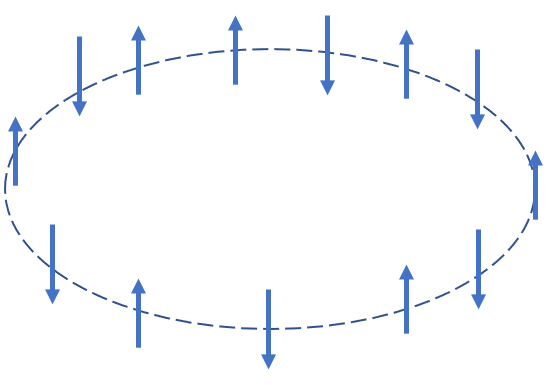
\includegraphics[scale=0.7]{periodic condition.png}
		\caption{Diagram of periodic boundary condition}
		\label{fig: periodic condition}
	\end{figure}
	
	In the code, two different initial conditions were used. The first was starting the simulations where all the spins were aligned randomly (``High" start). The second, was where all the spins were initially aligned (``Low" start). 
	
	\subsection{Calculating Variables}
	\label{subsubsec: calculateing variables}
	To research the properties of the system,we need to calculate several thermodynamic variables and investigate them. In particular, how they depend on the temperature of the system. From above content, we already know the analytic solutions of thermodynamic variables, but in the code, we have another way to calculate them.
	
	The average energy per spin is
	\begin{align}\label{equ: average energy per spin}
		\braket{E}=\frac{1}{2}\braket{H}=\frac{1}{2}\frac{-J \sum_{i=0}^{N-1} \sigma_i \sigma_{i+1}}{N}
	\end{align}
	
	For 1D lattice, the expect value of $\braket{E}$ is $-J$ when the spins are all aligned.
	
	The average magnetism per spin is 
	\begin{align}\label{equ: average magnetization per spin}
		\braket{M}=\frac{1}{N}\sum_{i=0}^{N-1} \sigma_i
	\end{align}
	
	The specific heat capacity $C_V$ is 
	\begin{align}\label{equ: spefic heat capacity}
		C_V=\frac{\partial \braket{E}}{\partial T}=-\frac{\beta}{T} \frac{\partial \braket{E}}{\partial \beta}=\frac{\beta}{T}\frac{\partial ^2 \ln(Z)}{\partial \beta ^2}=\frac{\beta}{T}\big(\braket{E^2}-\braket{E}^2\big)
	\end{align}
	
	The magnetic susceptibility is 
	\begin{align}\label{equ: susceptibility}
		\chi=\frac{\partial \braket{M}}{\partial H}=\beta \big(\braket{M^2}-\braket{M}^2 \big)
	\end{align}
	
	\section{Results}
	\label{sec: results}
	\subsection{Ferromagnet (J=1)}
	\label{equ: results for ferromagnet}
	\subsubsection{Cold start}
	\label{equ: ferromagnet cold start}
	
	In the simulation, the number of the spins is $N=100$, the evolution time steps is 1000, and the temperature's variation range is from 0 to 10 ($J/k_B$).The evolution for the 1D ising model with $h=0$ are shown in figures \ref{fig: configuration cold start T=1}. We can clearly see there is no phase transition which fits our discussion at section \ref{sec: phase transition}.
	
	For the plot of the average energy against temperature in figure \ref{fig: cold start average energy}, the basic trend was as expected compared with analytic solution: figure \ref{fig: analytic solution as temperature}. As the temperature increase, the energy of the system slowly began to increase. This is because as the temperature increase, thermal effects become more and more important and the system wants to go to the most entropically favourable state. 
	\begin{figure}[H]
		\centering
		\subfloat{\includegraphics[scale=0.5]{configuration (J=1,N=100, Low, T=1).pdf}} \quad
		\subfloat{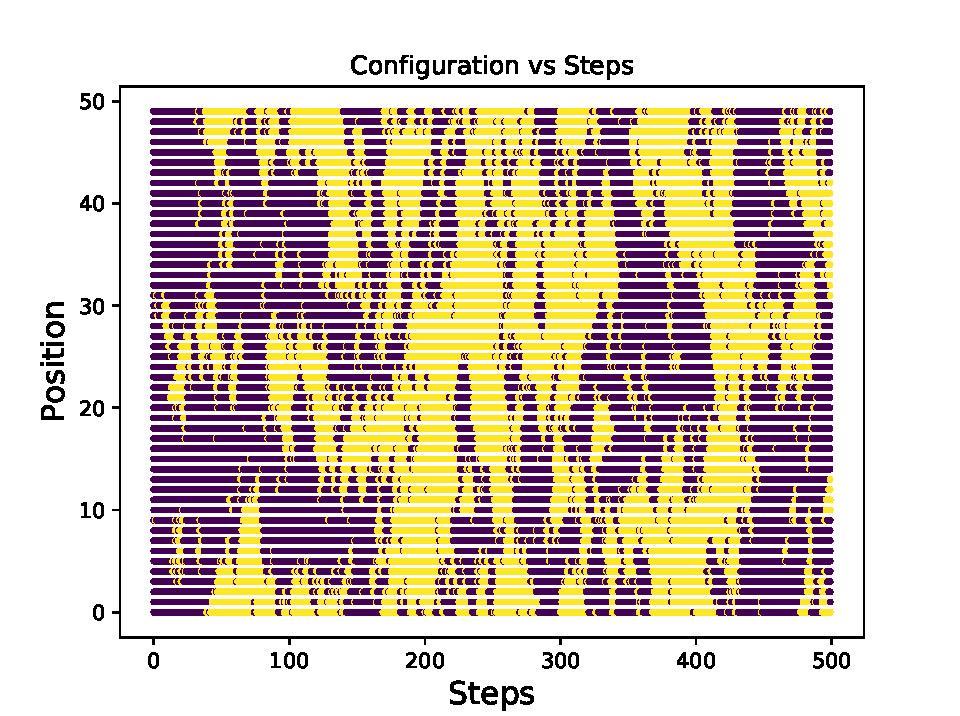
\includegraphics[scale=0.5]{configuration(J=1, N=50, Low, T=1).pdf}}
		\caption{Configuration vs Steps (Evolution time) at $T=1$, To make it more clear, the right picture is the amplification of the left one's some region.}
		\label{fig: configuration cold start T=1}
	\end{figure}
	
	Looking at the plot of the average magnetization against temperature (figure \ref{fig: cold start average magnetization}), the diagram is what we have seen at figure \ref{fig: analytic solution as temperature}. When temperatures changes from  0 to 10, the magnetization of the system is very close to zero. This makes sense because the 1D Ising model is not supposed to have a phase transition, and the material is supposed to be paramagnetic. When $T$ is lower than 1, the $\braket{M} \approx 1$ , so there appears to be a phase transition somewhere around here. Since it is well known from Ernst Ising’s solution that there should be no phase transition in the 1D ising model, what is causing this? It turns out that at very low temperatures the Metropolis algorithm fails to give a very physical representation of the system. The way the Metropolis algorithm determines whether or not to flip a spin when $dE>0$ is by comparing a random number to the Boltzmann factor (here $k_B=1$). But as $T\to 0$, we have 
	\begin{align*}
		\lim_{T \to 0} e^{-dE/{k_B T}}=0
	\end{align*}
	So when temperature is close to 0, the Metropolis algorithm will only flip spins so they align, but will never flip them out of alignment. This is why for very low temperatures the magnetization is always $\braket{M}=1$ and also for extremely low temperatures the energy is always $\braket{E}=-1$ which is the energy of the system when all the spins are aligned. To verify that, we have two more evolution plots for $T=1.2,0.8,0.6$ besides default $T=1$. We can easily see when $T$ is close to zero, there will be less magnetic domains which means it close to happen phase transition.
	
	\begin{figure}[H]
		\centering
		\subfloat[$T=1.2$]{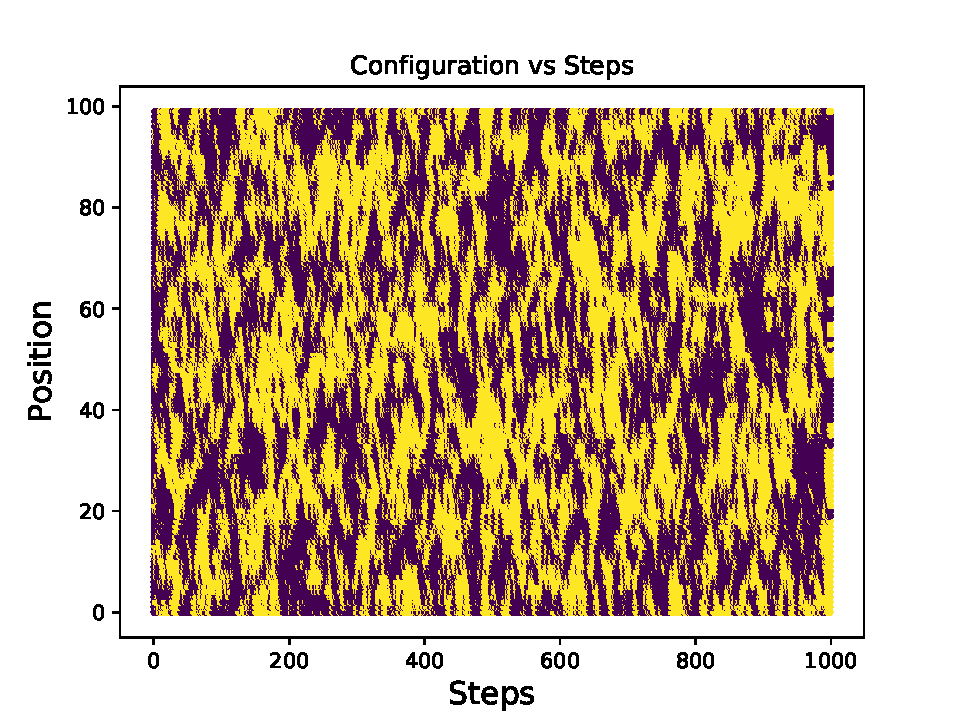
\includegraphics[scale=0.5]{configuration(J=1,N=100,Low,T=1.2).pdf}} \quad
		\subfloat[$T=1$]{\includegraphics[scale=0.5]{configuration (J=1,N=100, Low, T=1).pdf}} \quad
		\subfloat[$T=0.8$]{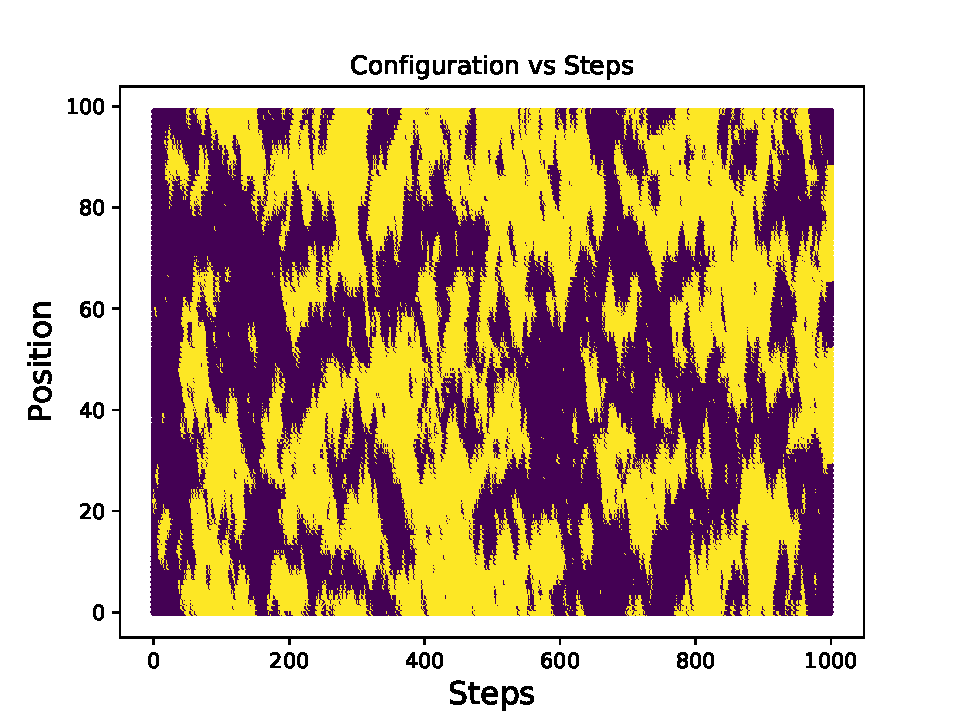
\includegraphics[scale=0.5]{configuration(J=1,N=100,Low,T=0.8).pdf}} \quad
		\subfloat[$T=0.6$]{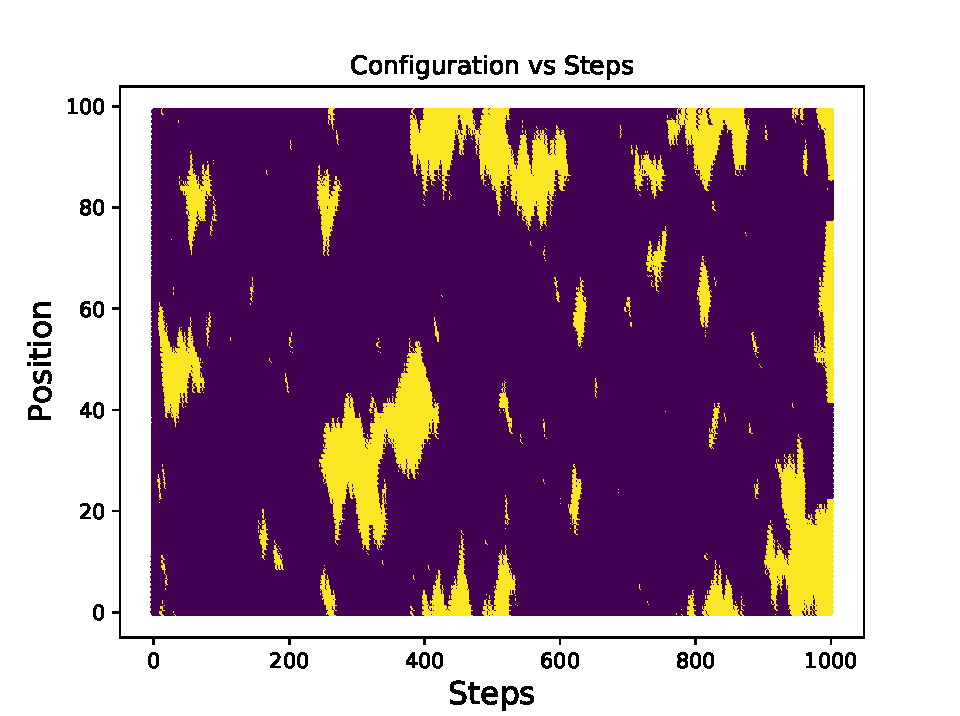
\includegraphics[scale=0.5]{configuration(J=1,N=100,Low,T=0.6).pdf}} 
		\caption{Different evolution with temperature changing.}
		\label{fig: evolution for differnet temperature}
	\end{figure}
	
	\begin{figure}[H]
		\begin{minipage}[t]{0.5\textwidth}
			\centering
			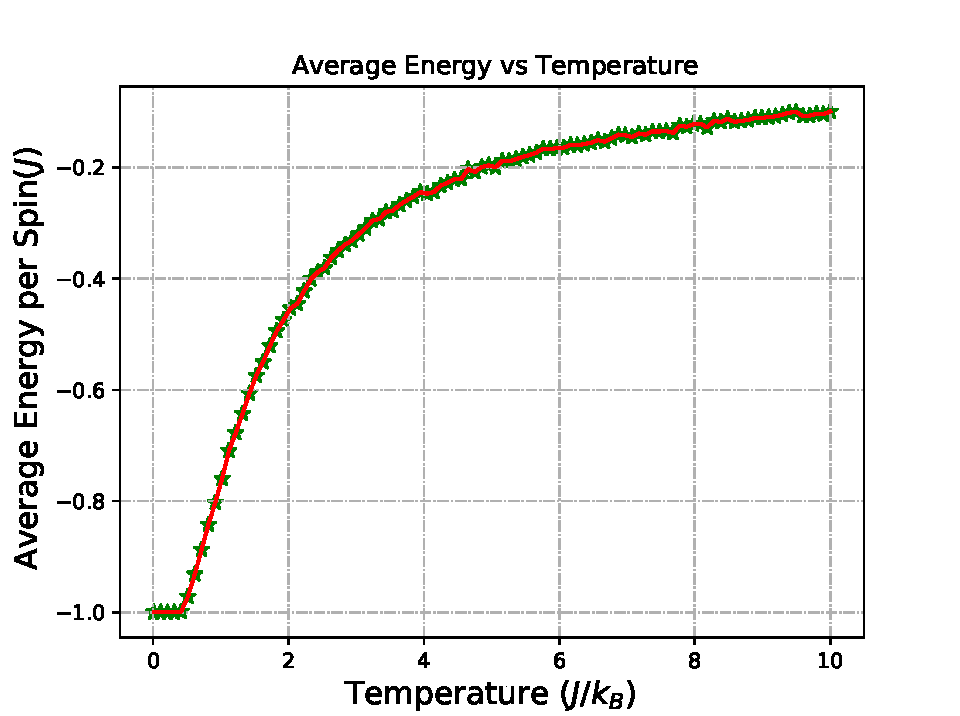
\includegraphics[scale=0.5]{ave E vs T(J=1).pdf}
			\setcaptionwidth{3in}
			\caption{$\braket{E}$ vs T for ``cold start"  ferromagnets (J=1). }
			\label{fig: cold start average energy}
		\end{minipage}
		\begin{minipage}[t]{0.5\textwidth}
			\centering
			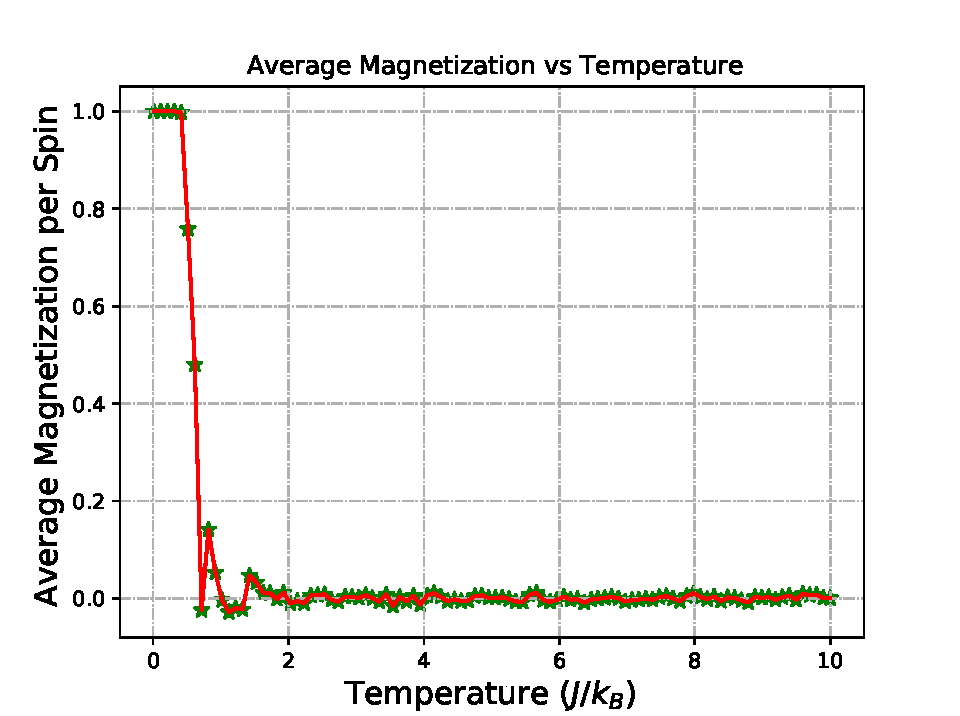
\includegraphics[scale=0.5]{ave M vs T(J=1).pdf}
			\setcaptionwidth{3in}
			\caption{$\braket{M}$ vs T for ``cold start"  ferromagnets (J=1).}
			\label{fig: cold start average magnetization}
		\end{minipage}
	\end{figure}
	
	\begin{figure}[H]
		\begin{minipage}[t]{0.5\textwidth}
			\centering
			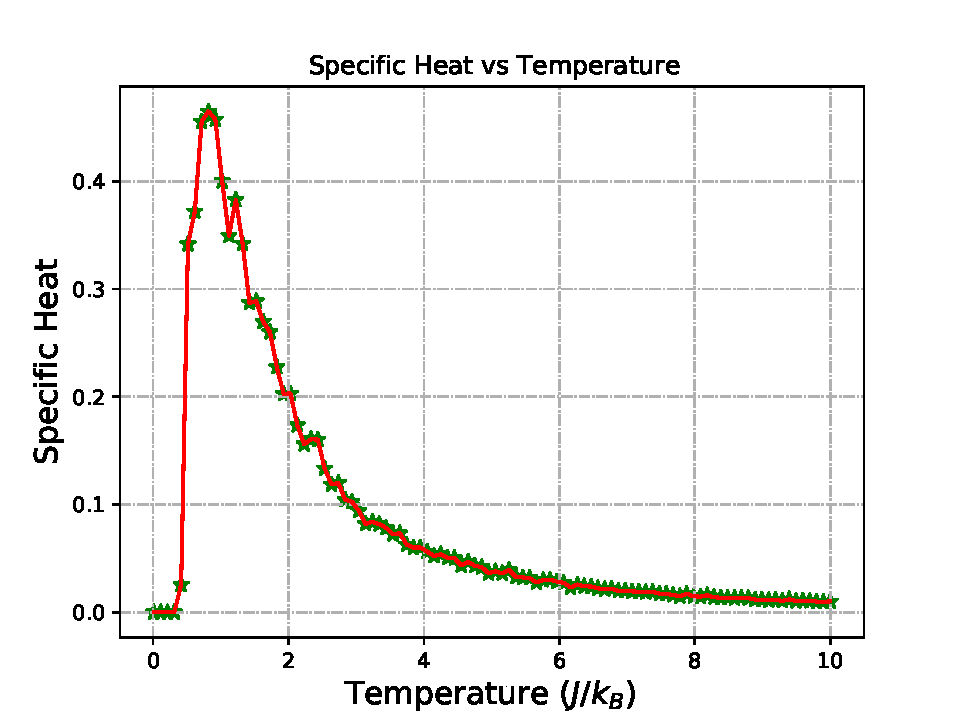
\includegraphics[scale=0.5]{C vs T (J=1).pdf}
			\setcaptionwidth{3in}
			\caption{C vs T for ``cold start"  ferromagnets (J=1). }
			\label{fig: cold start specific heat}
		\end{minipage}
		\begin{minipage}[t]{0.5\textwidth}
			\centering
			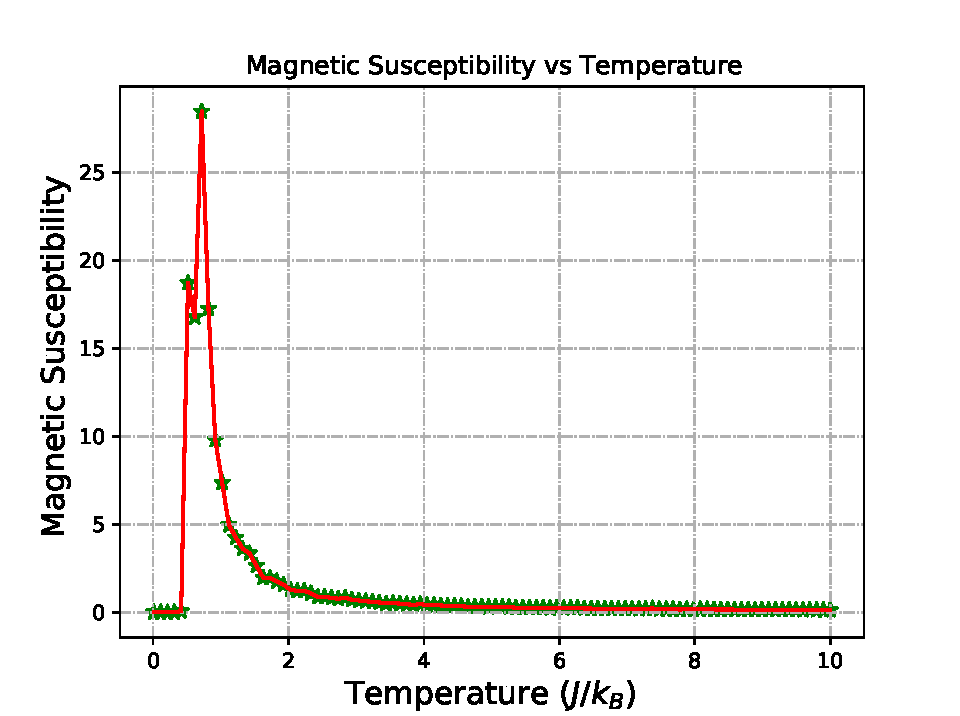
\includegraphics[scale=0.5]{X vs T (J=1).pdf}
			\setcaptionwidth{3in}
			\caption{$\braket{M}$ vs T for ``cold start" ferromagnets (J=1).}
			\label{fig: cold start suspecibility}
		\end{minipage}
	\end{figure}
	
	The specific heat capacity and suspecibility's plots (figure \ref{fig: cold start specific heat} and \ref{fig: cold start suspecibility}) are also as what we expected compared with figure \ref{fig: analytic solution as temperature}.
	
	\subsubsection{Hot Start}
	\label{sec: ferromagnet hot start}
	The evolution of ``Hot start'' whose spins are randomly arranged is as following. We can easily see there is no phase transition happen. 
	\begin{figure}[H]
		\centering
		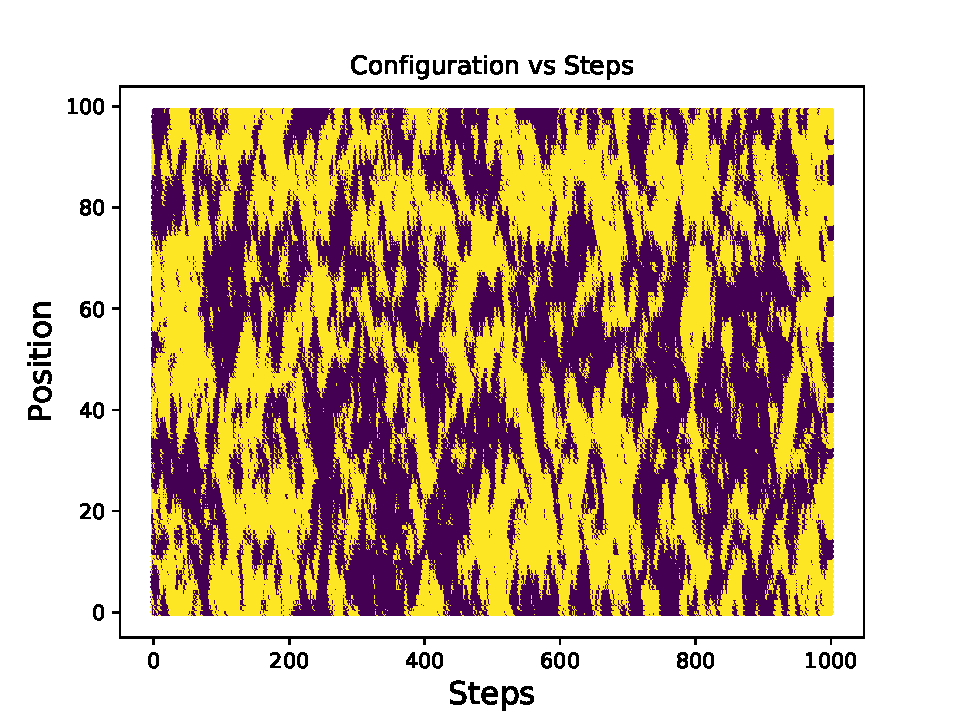
\includegraphics{configuration(J=1,N=100,High,T=1).pdf}
		\caption{Diagram of ``Hot Start" evolution where $T=1$}
		\label{fig: high start ferromagnet evolution}
	\end{figure}
	
	And the other results $\braket{E},\braket{M},\chi,C_v$ are as following
	\begin{figure}[H]
		\begin{minipage}[t]{0.5\textwidth}
			\centering
			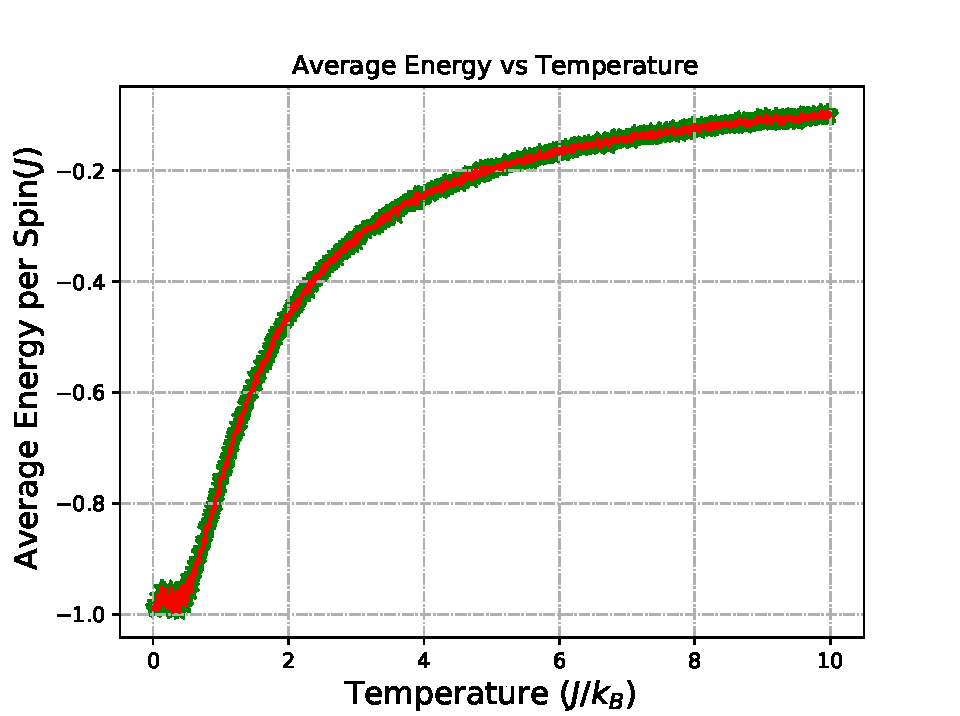
\includegraphics[scale=0.5]{ave E vs T (High, J=1).pdf}
			\setcaptionwidth{3in}
			\caption{$\braket{E}$ vs T for ``Hot start"  ferromagnets (J=1). }
			\label{fig: high start average energy}
		\end{minipage}
		\begin{minipage}[t]{0.5\textwidth}
			\centering
			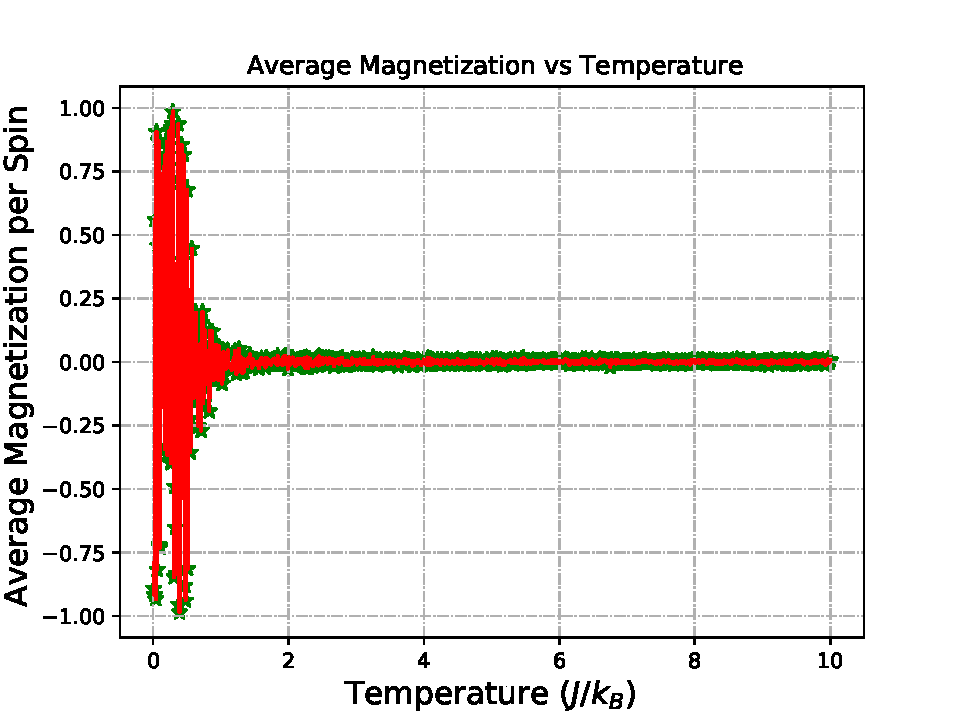
\includegraphics[scale=0.5]{ave M vs T(High, J=1).pdf}
			\setcaptionwidth{3in}
			\caption{$\braket{M}$ vs T for ``hot start"  ferromagnets (J=1).}
			\label{fig: high start average magnetization}
		\end{minipage}
	\end{figure}
	
	\begin{figure}[H]
		\begin{minipage}[t]{0.5\textwidth}
			\centering
			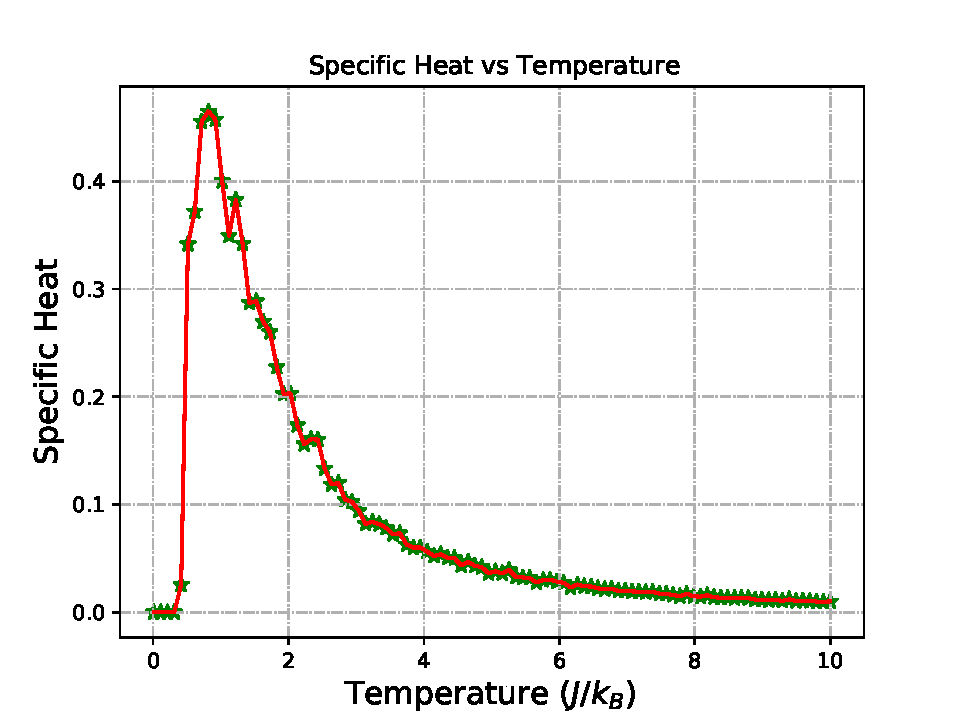
\includegraphics[scale=0.5]{C vs T (J=1).pdf}
			\setcaptionwidth{3in}
			\caption{C vs T for ``hot start"  ferromagnets (J=1). }
			\label{fig: high start specific heat}
		\end{minipage}
		\begin{minipage}[t]{0.5\textwidth}
			\centering
			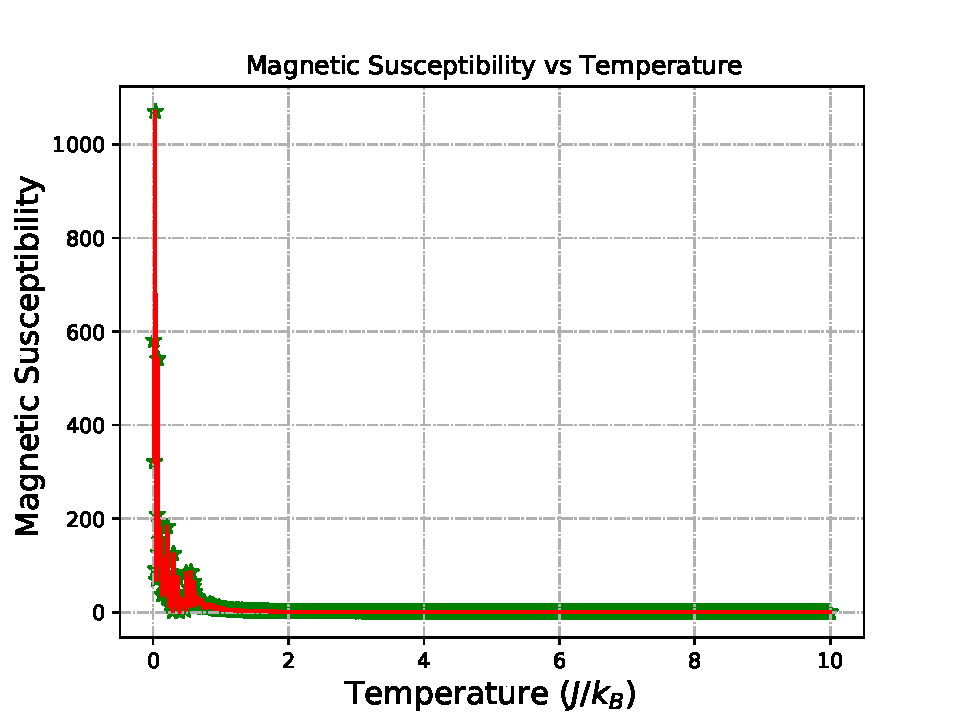
\includegraphics[scale=0.5]{X vs T (High, J=1).pdf}
			\setcaptionwidth{3in}
			\caption{$\braket{M}$ vs T for ``hot start" ferromagnets (J=1).}
			\label{fig: high start suspecibility}
		\end{minipage}
	\end{figure}
	
	\subsection{Antiferromagnet (J=-1)}
	\label{sec: results of antiferromagnet}
	In a ferromagnetic Ising model, spins desire to be aligned: the configurations in which adjacent spins are of the same sign have higher probability. In an antiferromagnetic model, adjacent spins tend to have opposite signs.  So the difference of ``cold start" and ``hot start'' for antiferromagnet is very small. Their plots are almost the same, therefore we only give ``cold start'' results.
	
	The results are as following 
	\begin{figure}[H]
		\centering
		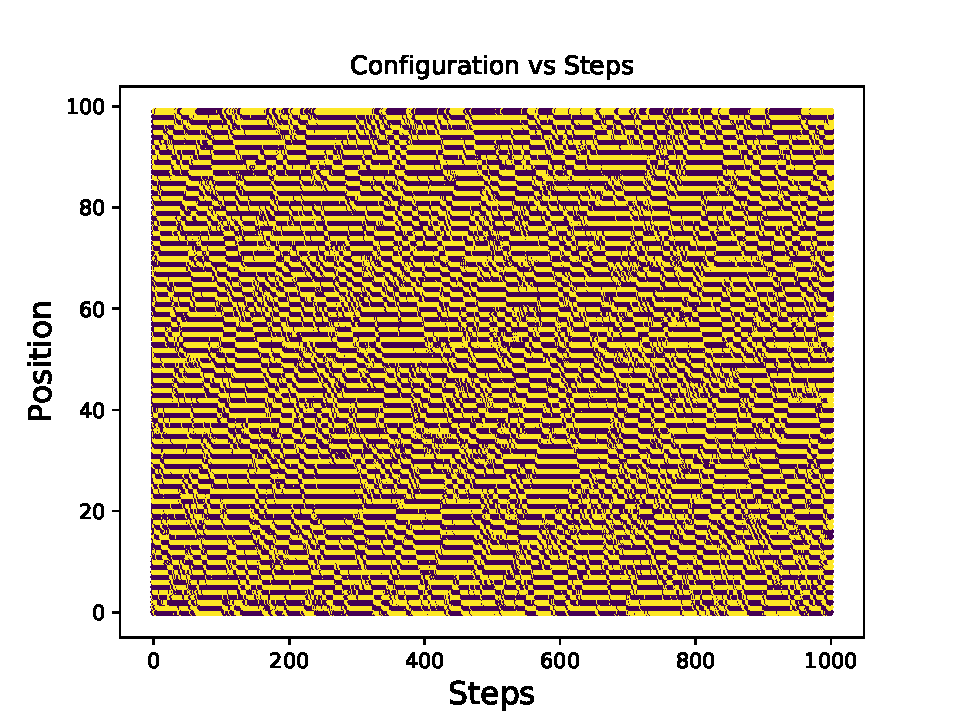
\includegraphics{configuration (J=-1,N=100,Low,T=1).pdf}
		\caption{Diagram of  evolution for antiferromagnet with $T=1$}
		\label{fig: evolution of antiferromagnet low start}
	\end{figure}
	
	\begin{figure}[H]
		\begin{minipage}[t]{0.5\textwidth}
			\centering
			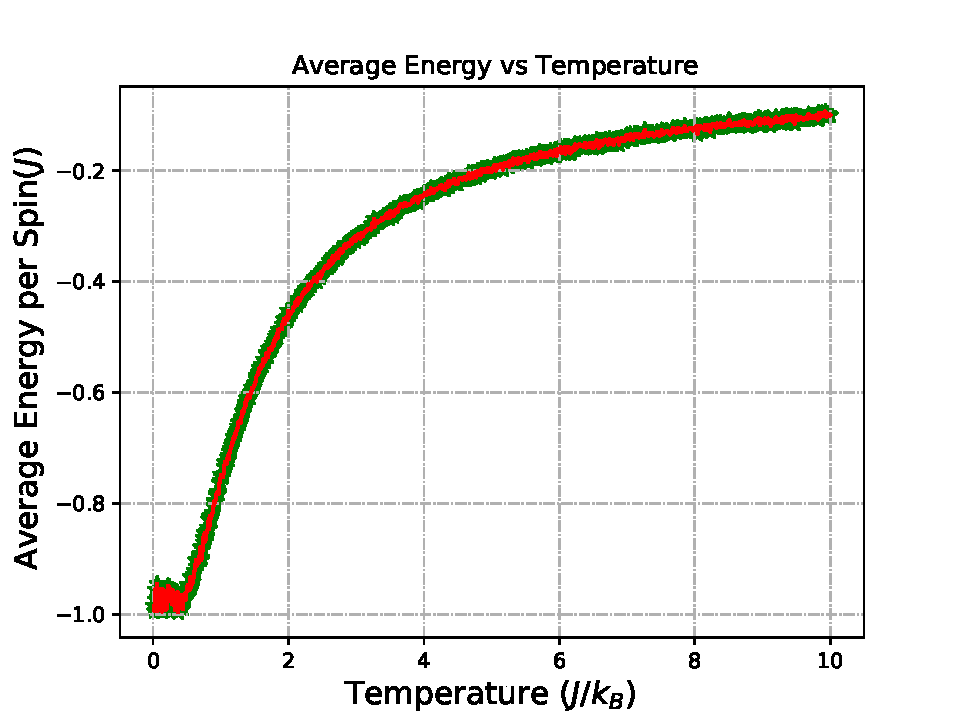
\includegraphics[scale=0.5]{ave E vs T (Low, J=-1).pdf}
			\setcaptionwidth{3in}
			\caption{$\braket{E}$ vs T for  antiferromagnets (J=-1). }
			\label{fig: low start average energy for antiferromagnet}
		\end{minipage}
		\begin{minipage}[t]{0.5\textwidth}
			\centering
			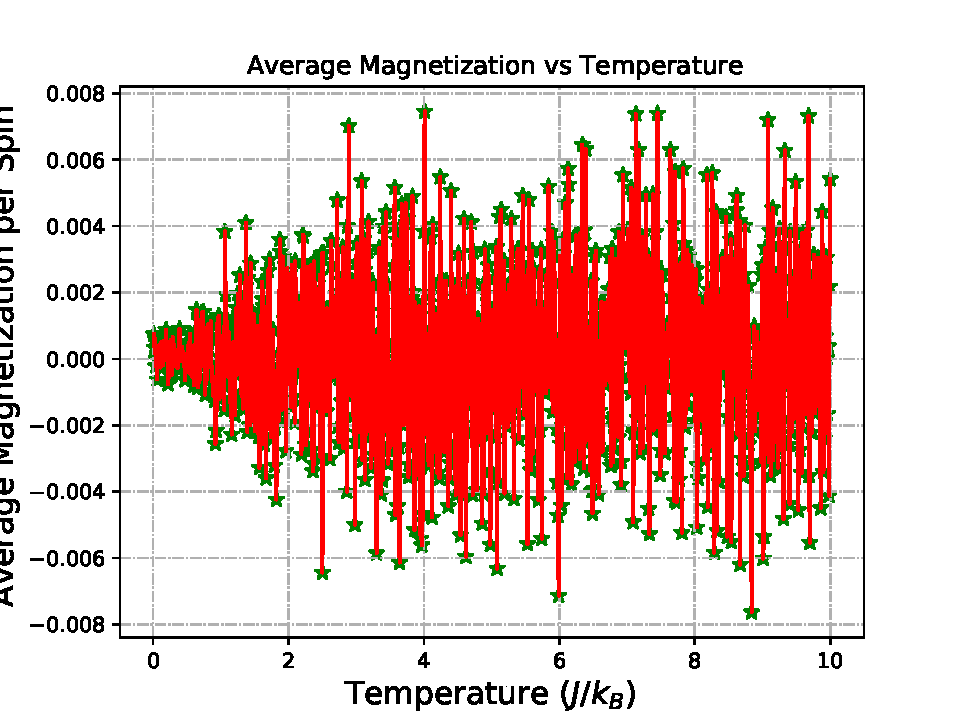
\includegraphics[scale=0.5]{ave M vs T (Low, J=-1).pdf}, 
			\setcaptionwidth{3in}
			\caption{$\braket{M}$ vs T for  antiferromagnets (J=-1).}
			\label{fig: low start average magnetization for antiferromagnet}
		\end{minipage}
	\end{figure}
	
	\begin{figure}[H]
		\begin{minipage}[t]{0.5\textwidth}
			\centering
			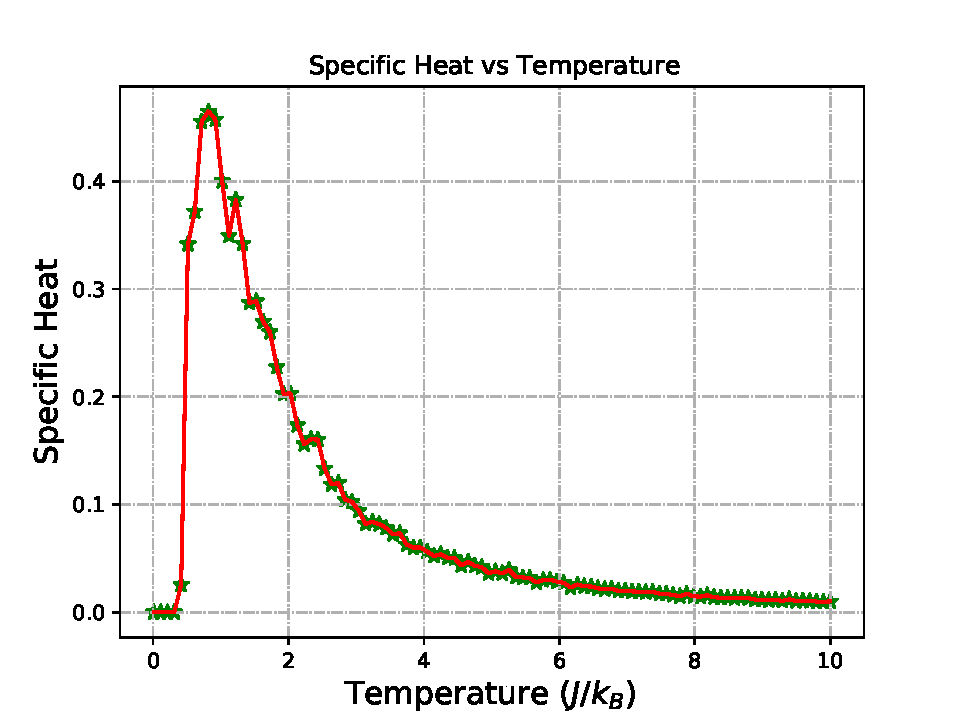
\includegraphics[scale=0.5]{C vs T (J=1).pdf}
			\setcaptionwidth{3in}
			\caption{C vs T for antiferromagnets (J=-1). }
			\label{fig: low start specific heat for antiferromagnet}
		\end{minipage}
		\begin{minipage}[t]{0.5\textwidth}
			\centering
			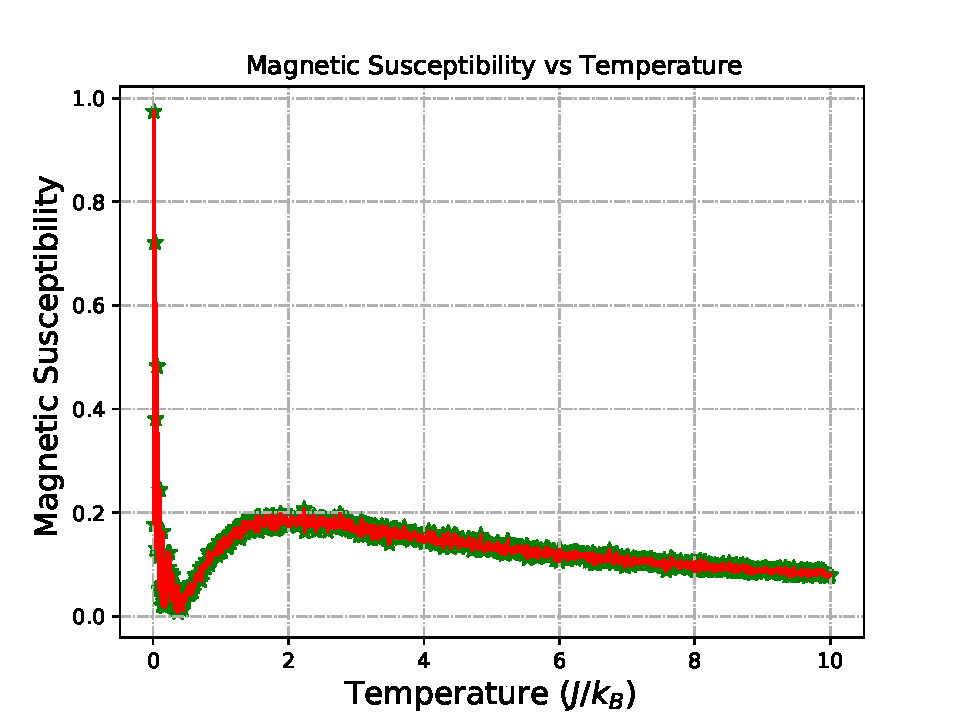
\includegraphics[scale=0.5]{X vs T (Low, J=-1).pdf}
			\setcaptionwidth{3in}
			\caption{$\braket{M}$ vs T for antiferromagnets (J=-1).}
			\label{fig: low start suspecibility for antiferromagnet}
		\end{minipage}
	\end{figure}
	
	We can see the results are well matched with the second row of figure \ref{fig: analytic solution as temperature} except the $\braket{M}$. That is because we don't consider external field in the code, but the analytic solution of $\braket{M}$ depends on external field. 
	
	\subsection{Equilibrium of the System}
	\label{sec: equilibrium of system}
	As the system was sampled more and more, each individual spin
	was more likely to be in its most probable microstate.
	As more and more spins went to their most probable microstate, the overall system went to its most probable macrostate or the state the system will be in once its equilibrated. . As the system approaches this state, the fluctuations in the expectation values of thermodynamic quantities begins to decrease, and the decrease in these fluctuations was used as an indicator that the system
	had reached equilibrium. 
	
	For ``cold start'', we have the figure \ref{fig:cold start equilibrium} plots. It's easy to see when the temperature is higher, the $\braket{M}$ is tend to be more stable around 0, the number which means it reaches equilibrium.
	\begin{figure}[htb]
		\centering
		\subfloat[$T=0.1$]{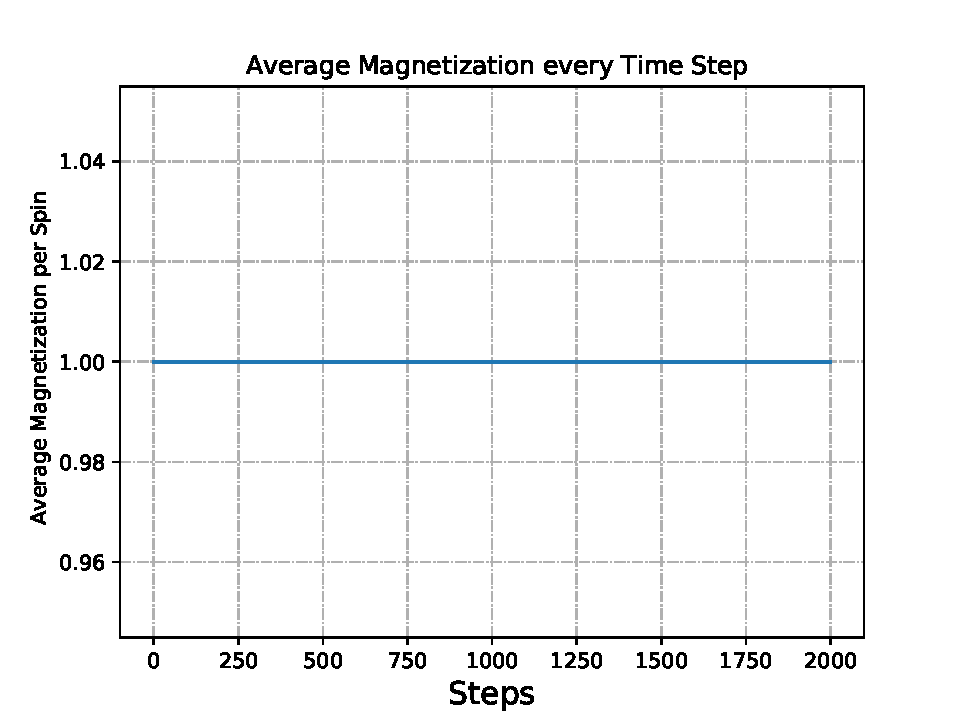
\includegraphics[scale=0.45]{equ (T=0.1, J=1).pdf}} \quad
		\subfloat[$T=0.5$]{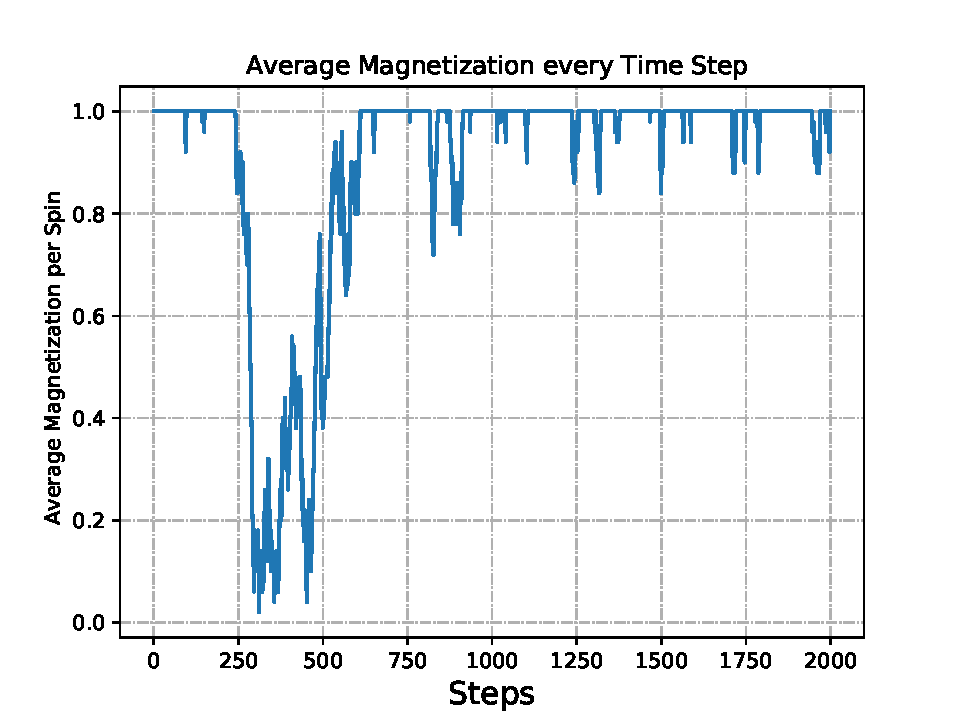
\includegraphics[scale=0.45]{equ (T=0.5, J=1).pdf}} \quad
		\subfloat[$T=1$]{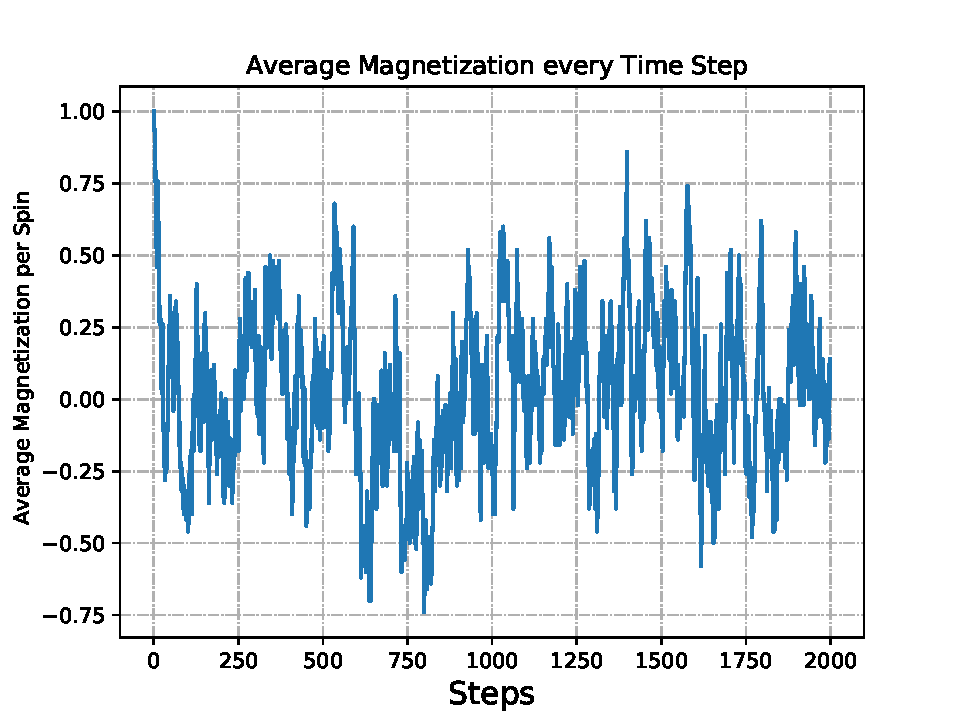
\includegraphics[scale=0.45]{equ (T=1, J=1).pdf}} \quad
		\subfloat[$T=5$]{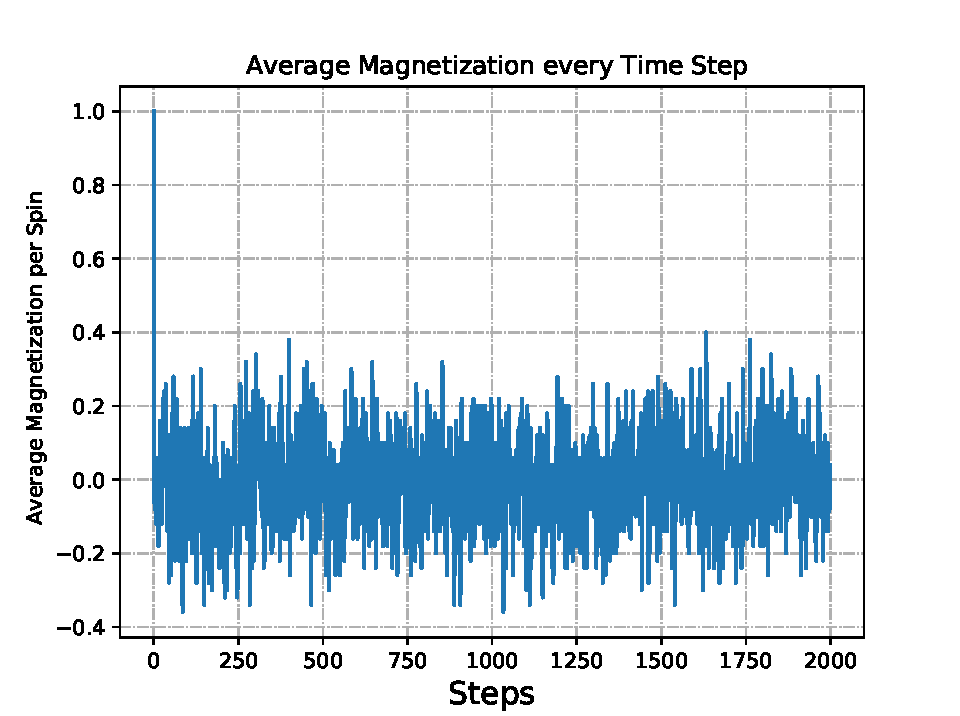
\includegraphics[scale=0.45]{equ (T=5, J=1).pdf}}
		\caption{$\braket{M}$ follows time steps for cold start}
		\label{fig:cold start equilibrium}
	\end{figure}
	
	The figure \ref{fig:hot start equilibrium} plots are hot start results.
	\begin{figure}[H]
		\centering
		\subfloat[$T=0.1$]{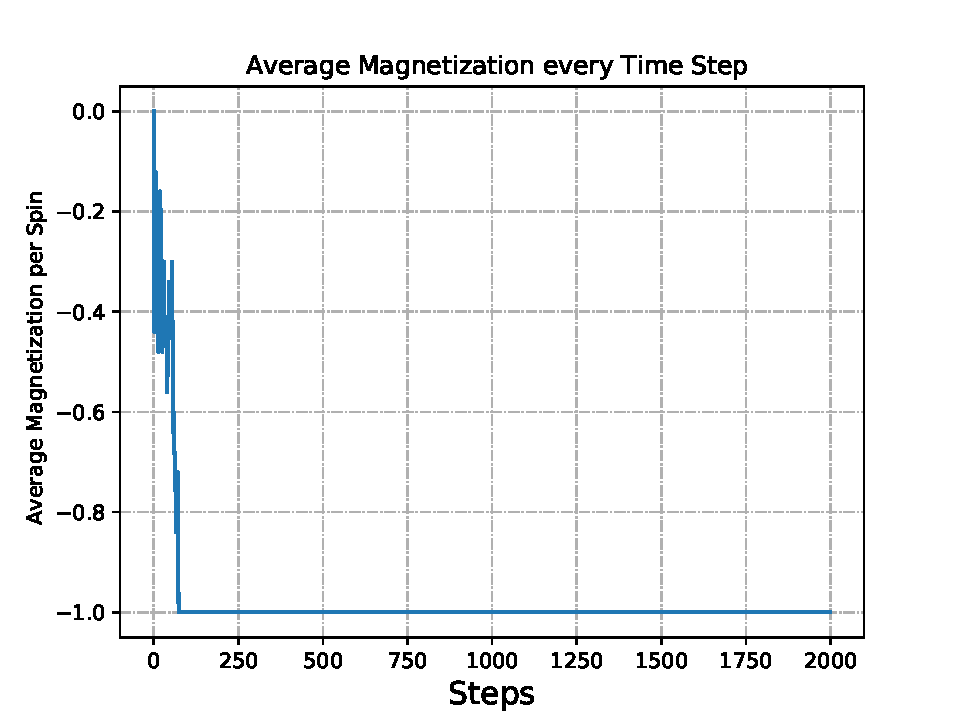
\includegraphics[scale=0.45]{equ (T=0.1, J=1, High).pdf}} \quad
		\subfloat[$T=0.5$]{\includegraphics[scale=0.45]{equ (T=0.5, J=1, High).pdf}} \quad
		\subfloat[$T=1$]{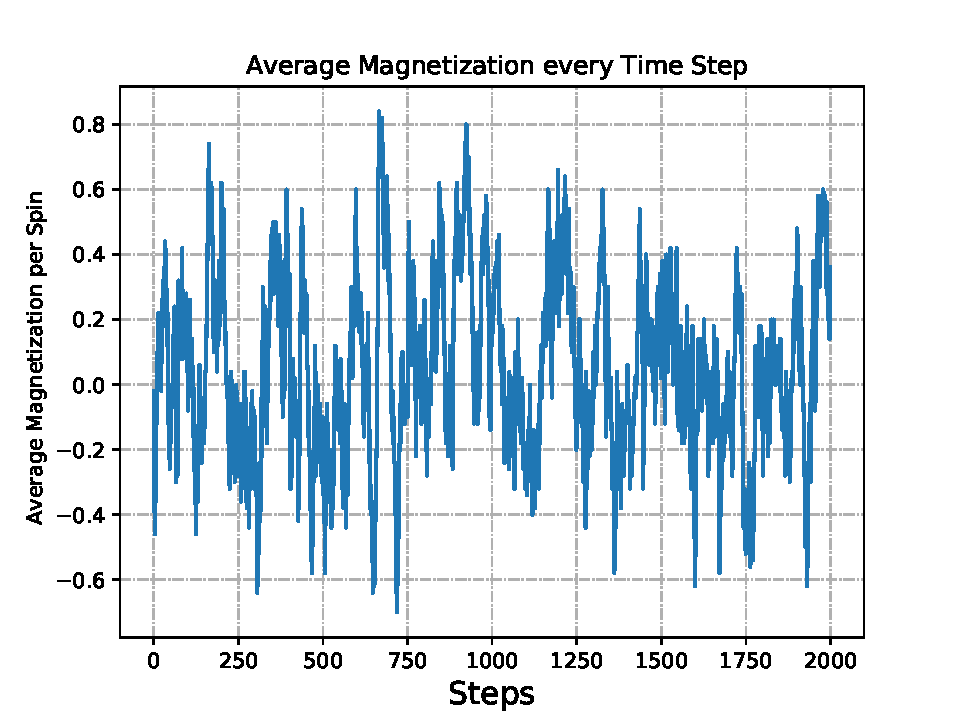
\includegraphics[scale=0.45]{equ (T=1, J=1, High).pdf}} \quad
		\subfloat[$T=5$]{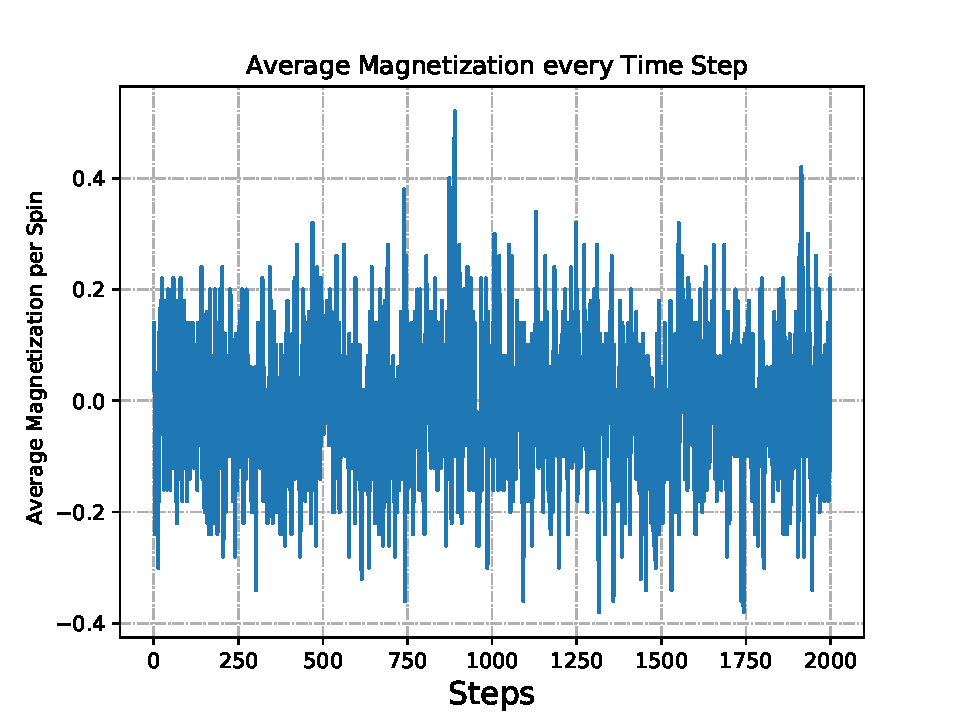
\includegraphics[scale=0.45]{equ (T=5, J=1, High).pdf}} \quad
		\caption{$\braket{M}$ follows time steps for hot start}
		\label{fig:hot start equilibrium}
	\end{figure}
	
	The plots are of ferromagnets, for antiferromagnets, the plots are almost the same style so we don't show them again.
	
	\section{Conclusion}
	\label{sec: conclusion}
	In this experiment Monte Carlo simulations were created of the 1D and Ising model. To do this the Metropolis algorithm was implemented in Python. The dependence of the energy, magnetization, specific heat, and magnetic susceptibility of the system on temperature were calculated for the 1D and Ising model. Some simple tests were done to try to understand the effects of increasing the amount of sampling and the system size in Monte Carlo simulations. The experiment was a success in that we learned some of the basics of how to run simulations and achieved results
	that were comparable to the analytic solution. 
	
	\begin{thebibliography}{99}
		\bibitem{wikipedia ising model}
		Wikipeida: \url{https://en.wikipedia.org/wiki/Ising_model#One_dimension}
		\bibitem{wikipedia magnetic domain}
		Wikipeida: \url{https://en.wikipedia.org/wiki/Magnetism#Magnetic_domains}
		\bibitem{1d simulation paper}
		Asher Preska Steinberg, Michael Kosowsky and Seth Fraden, \textit{Simulations: The Ising Model}
		\bibitem{statistical physics book}
		David Chandler, \textit{Introduction To Modern Statistical Mechanics}
		\bibitem{lecture note}
		Lecture 9 Note: \url{https://lemida.biu.ac.il/pluginfile.php/1638312/mod_resource/content/0/Lecture09%2B10-moodle.pdf}
		\end{thebibliography}
		
	\end{document}
